\part{AI, ethics and society}
\frame{\partpage}

\begin{frame}{Some ethical issues around AI}
	\begin{itemize}
		\pause\item Bias in, bias out
			\begin{itemize}
				\pause\item E.g.\ Google Translate
			\end{itemize}
		\pause\item Bias inherited from tech industry
			\begin{itemize}
				\pause\item E.g.\ facial recognition struggling with non-Caucasian faces
			\end{itemize}
		\pause\item Bias caused by deliberate manipulation of training data
			\begin{itemize}
				\pause\item E.g.\ Microsoft Tay chatbot
			\end{itemize}
		\pause\item Privacy, security and safety
		\pause\item Public perception (trust or mistrust) of AI
		\pause\item Responsibility for AI's actions
		\pause\item Automation of jobs
	\end{itemize}
\end{frame}

\begin{frame}{Money laundering for bias}

``Instead of relying on algorithms, which we can be accused of manipulating for
our benefit, we have turned to machine learning, an ingenious way of disclaiming
responsibility for anything. Machine learning is like money laundering for bias.
It's a clean, mathematical apparatus that gives the status quo the aura of
logical inevitability. The numbers don't lie.''

--- Maciej Ceg\l{}owski

{\tiny\url{http://idlewords.com/talks/sase_panel.htm}}
\end{frame}

\begin{frame}
	\begin{center}
		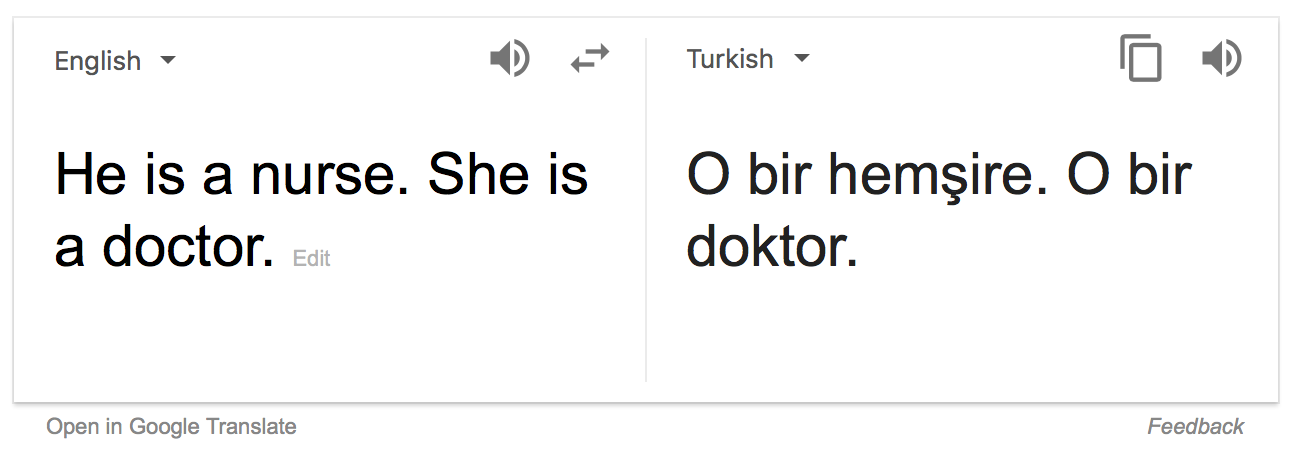
\includegraphics[width=\textwidth]{translate1}
	\end{center}
	\begin{center}
		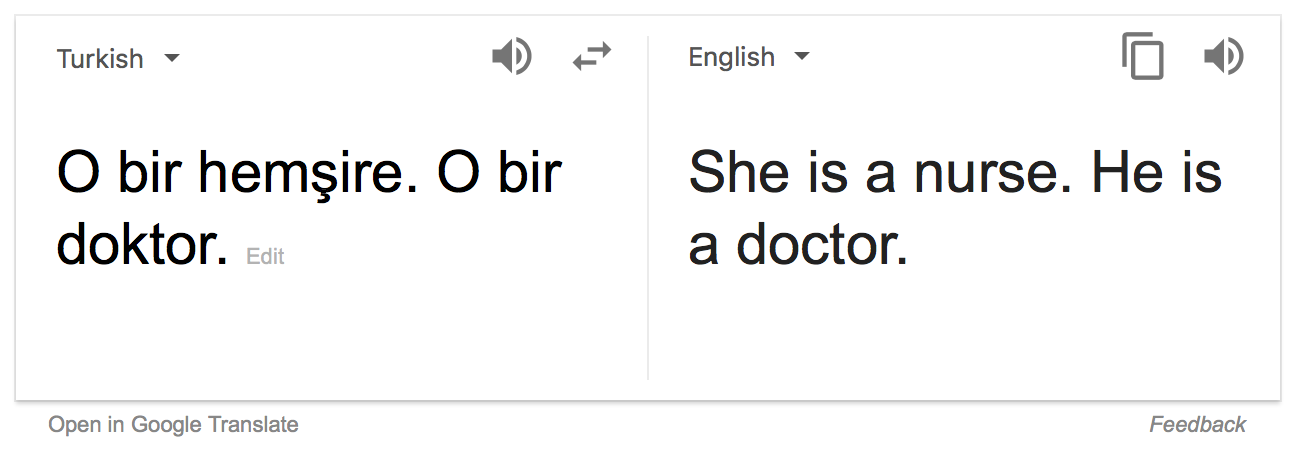
\includegraphics[width=\textwidth]{translate2}
	\end{center}
\end{frame}

\begin{frame}
	\begin{center}
		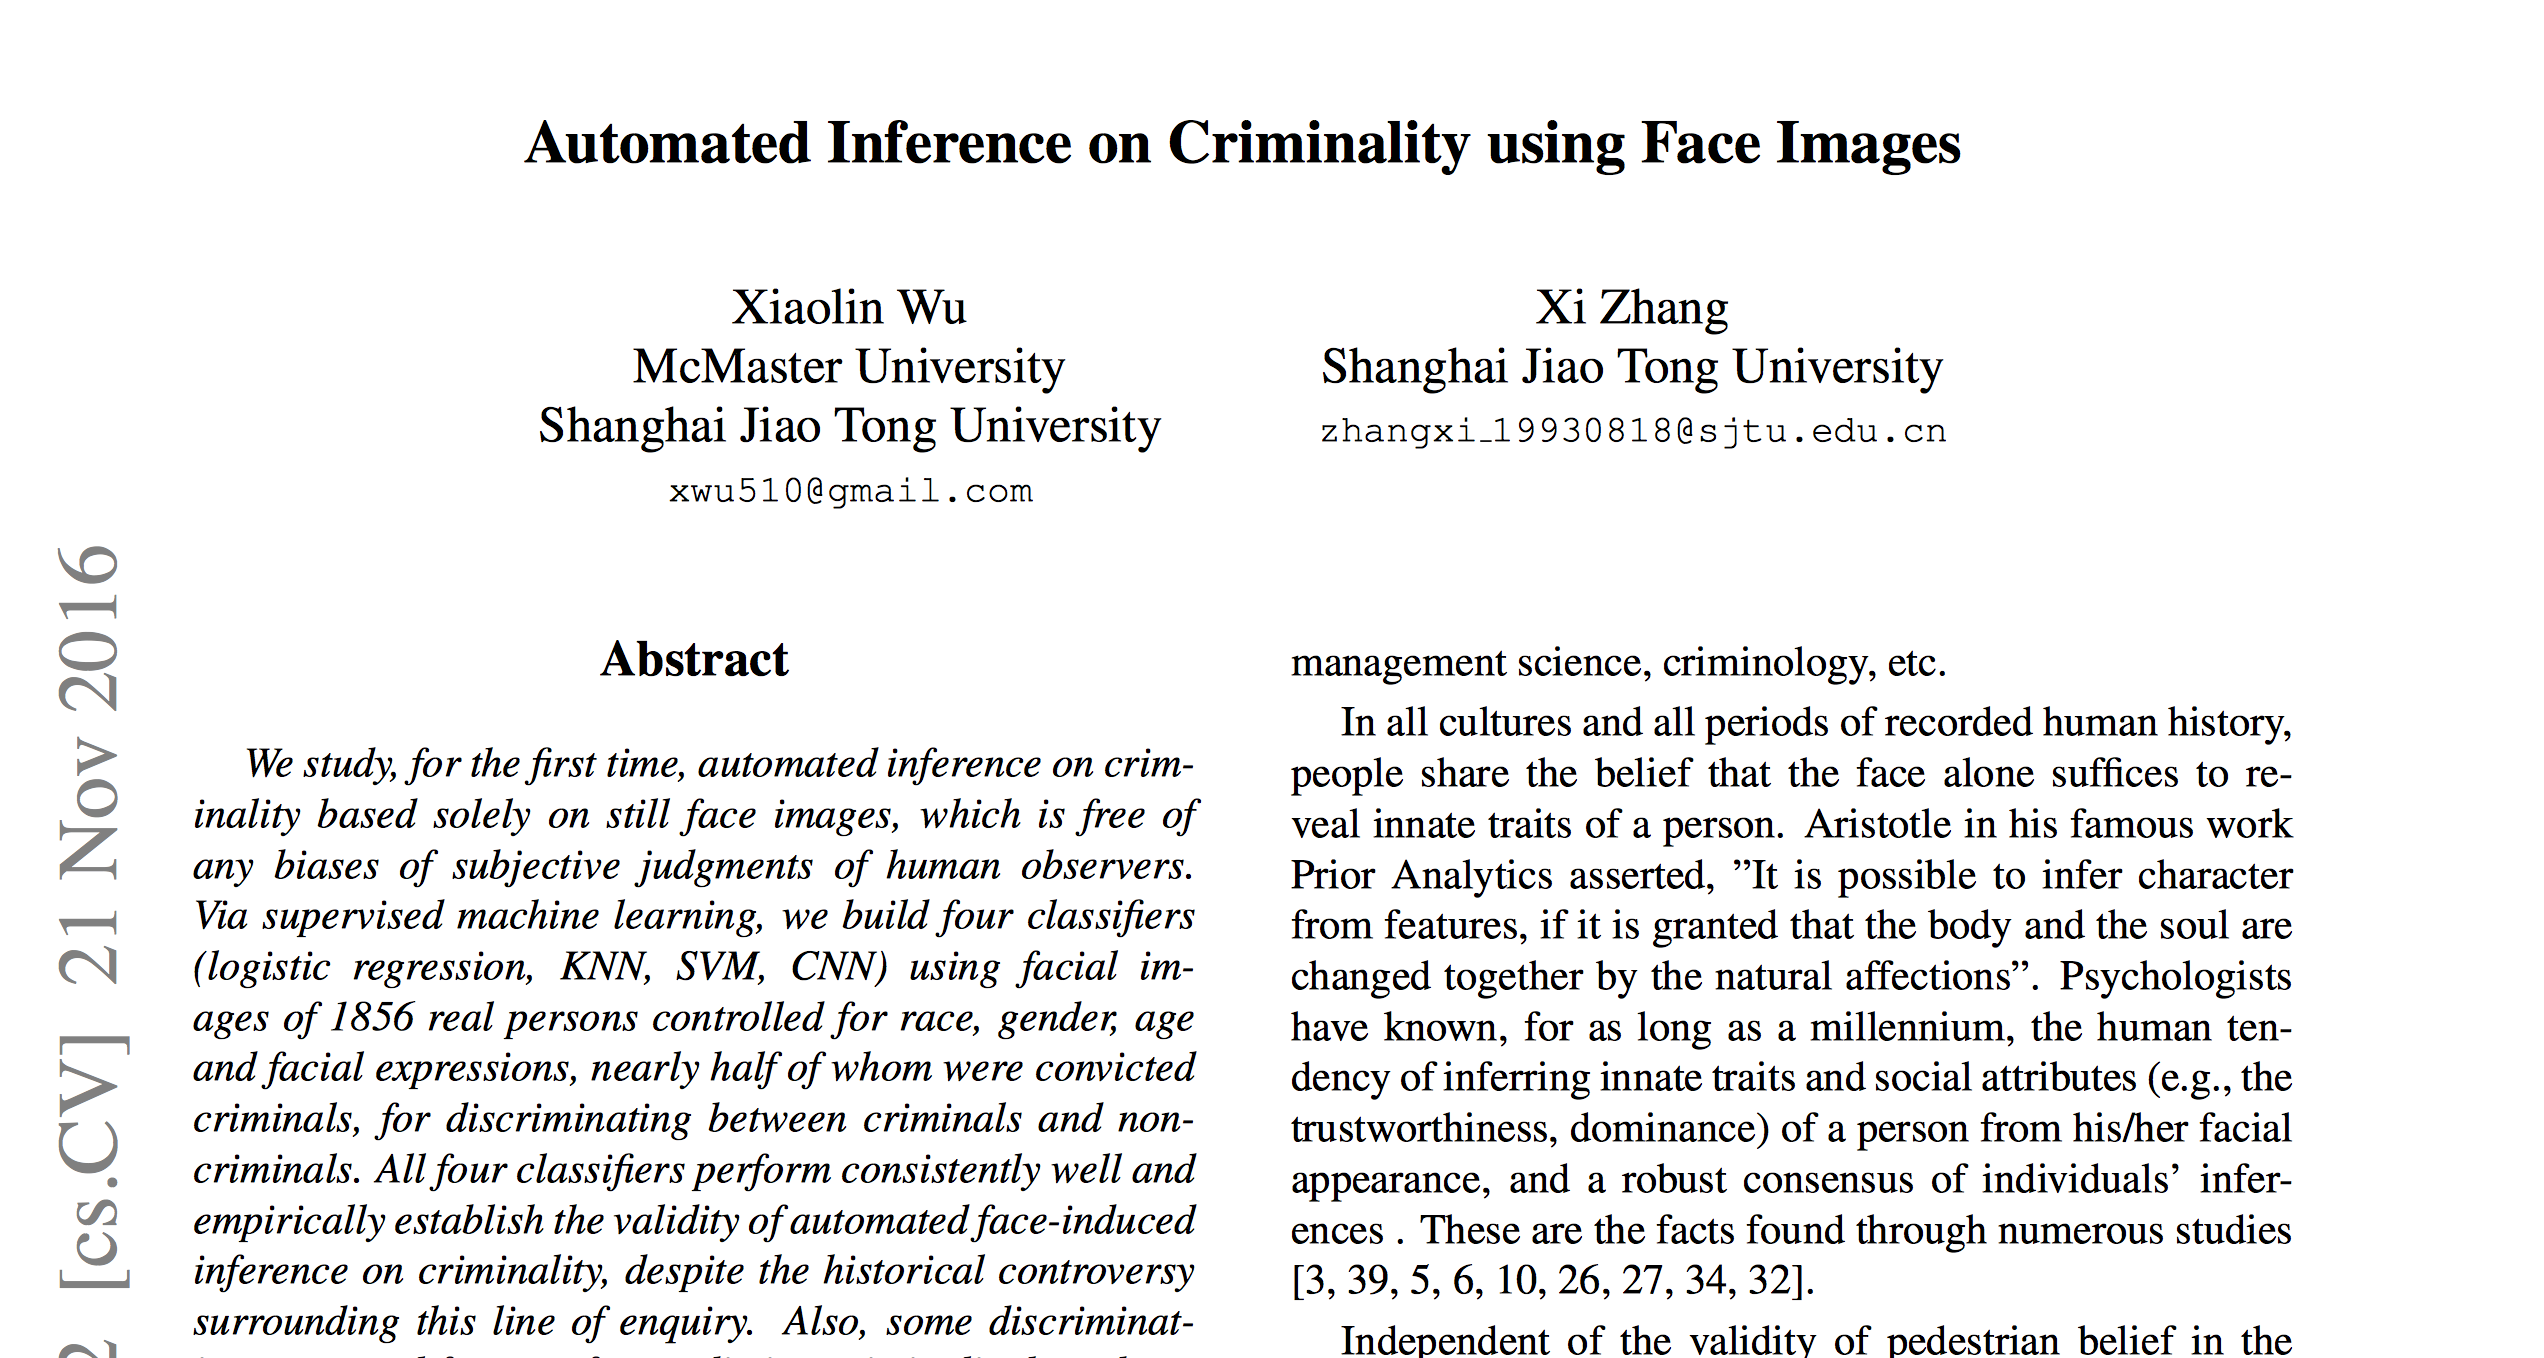
\includegraphics[width=\textwidth]{criminality1}
	\end{center}
\end{frame}

\begin{frame}
	\begin{center}
		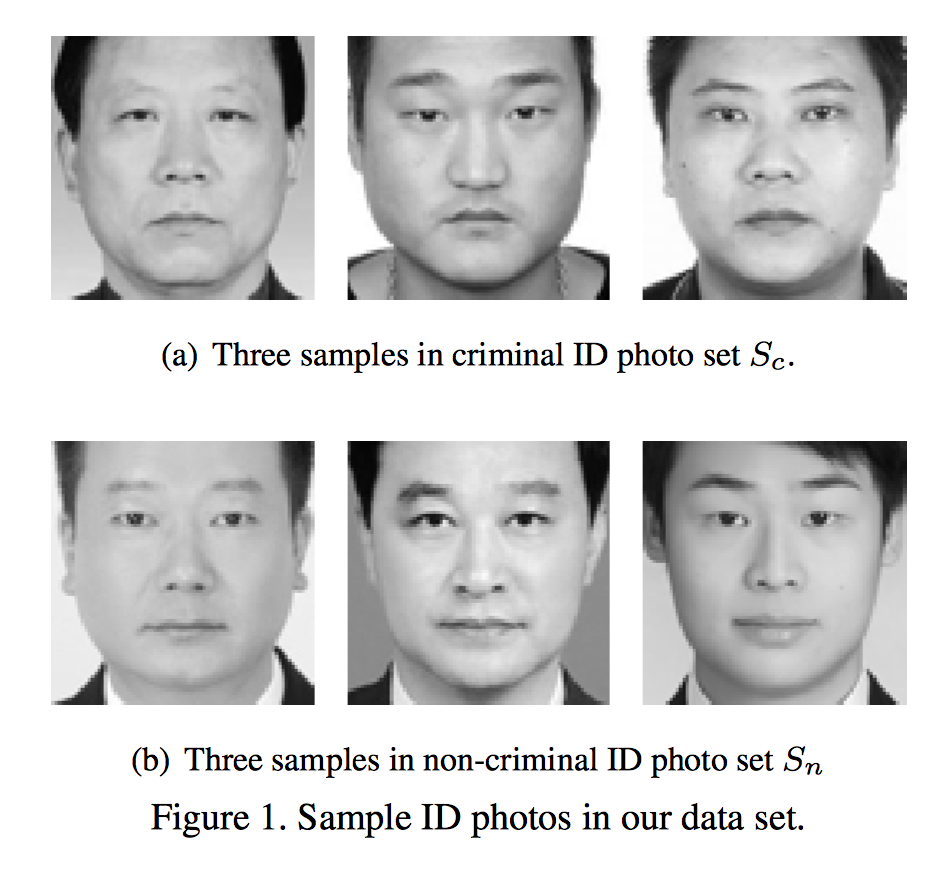
\includegraphics[height=0.6\textheight]{criminality2}
	\end{center}
\end{frame}

\begin{frame}
	\begin{center}
		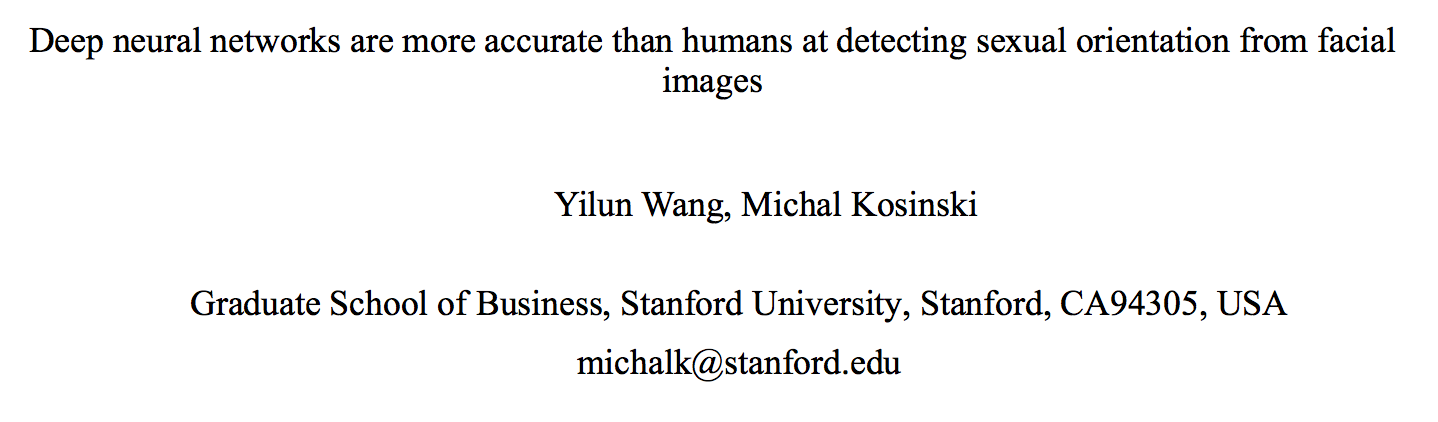
\includegraphics[width=\textwidth]{orientation1}
	\end{center}
\end{frame}

\begin{frame}
	\begin{center}
		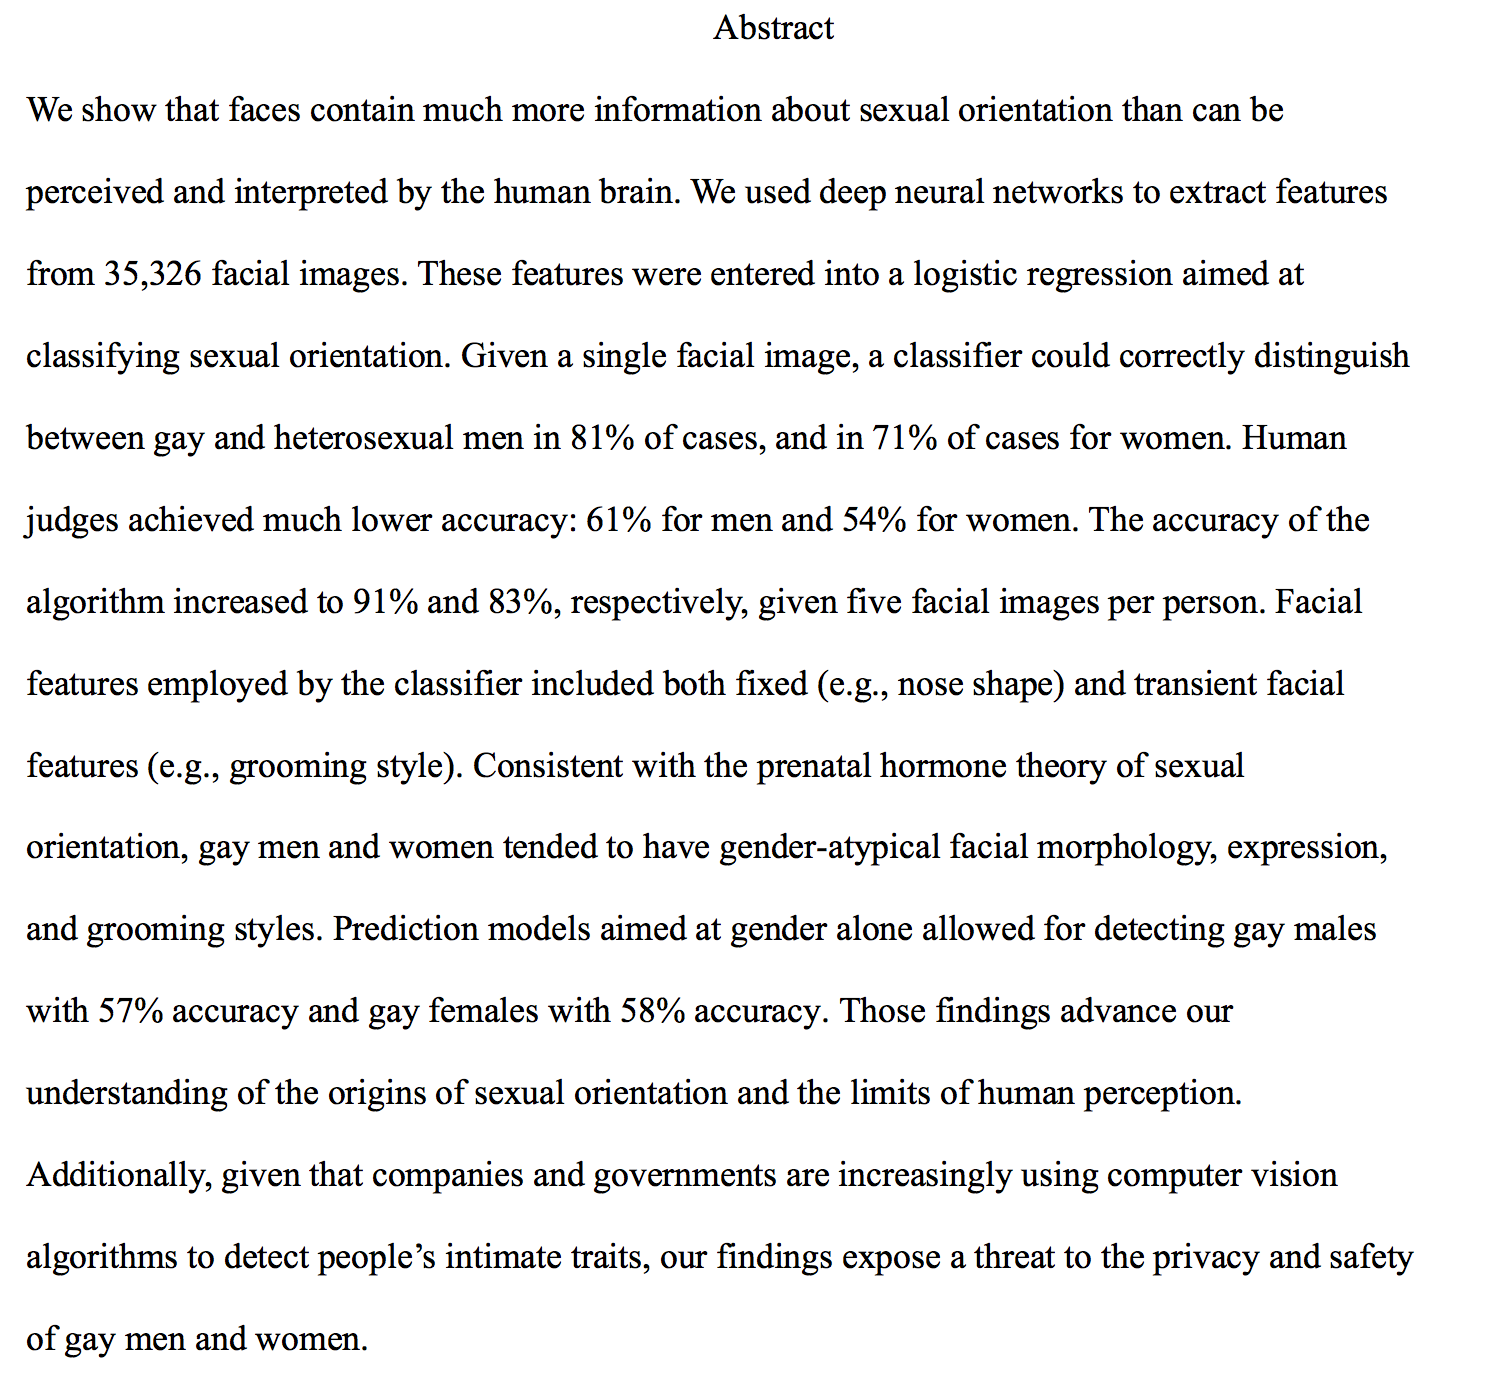
\includegraphics[height=0.8\textheight]{orientation2}
	\end{center}
\end{frame}

\begin{frame}
	\begin{center}
		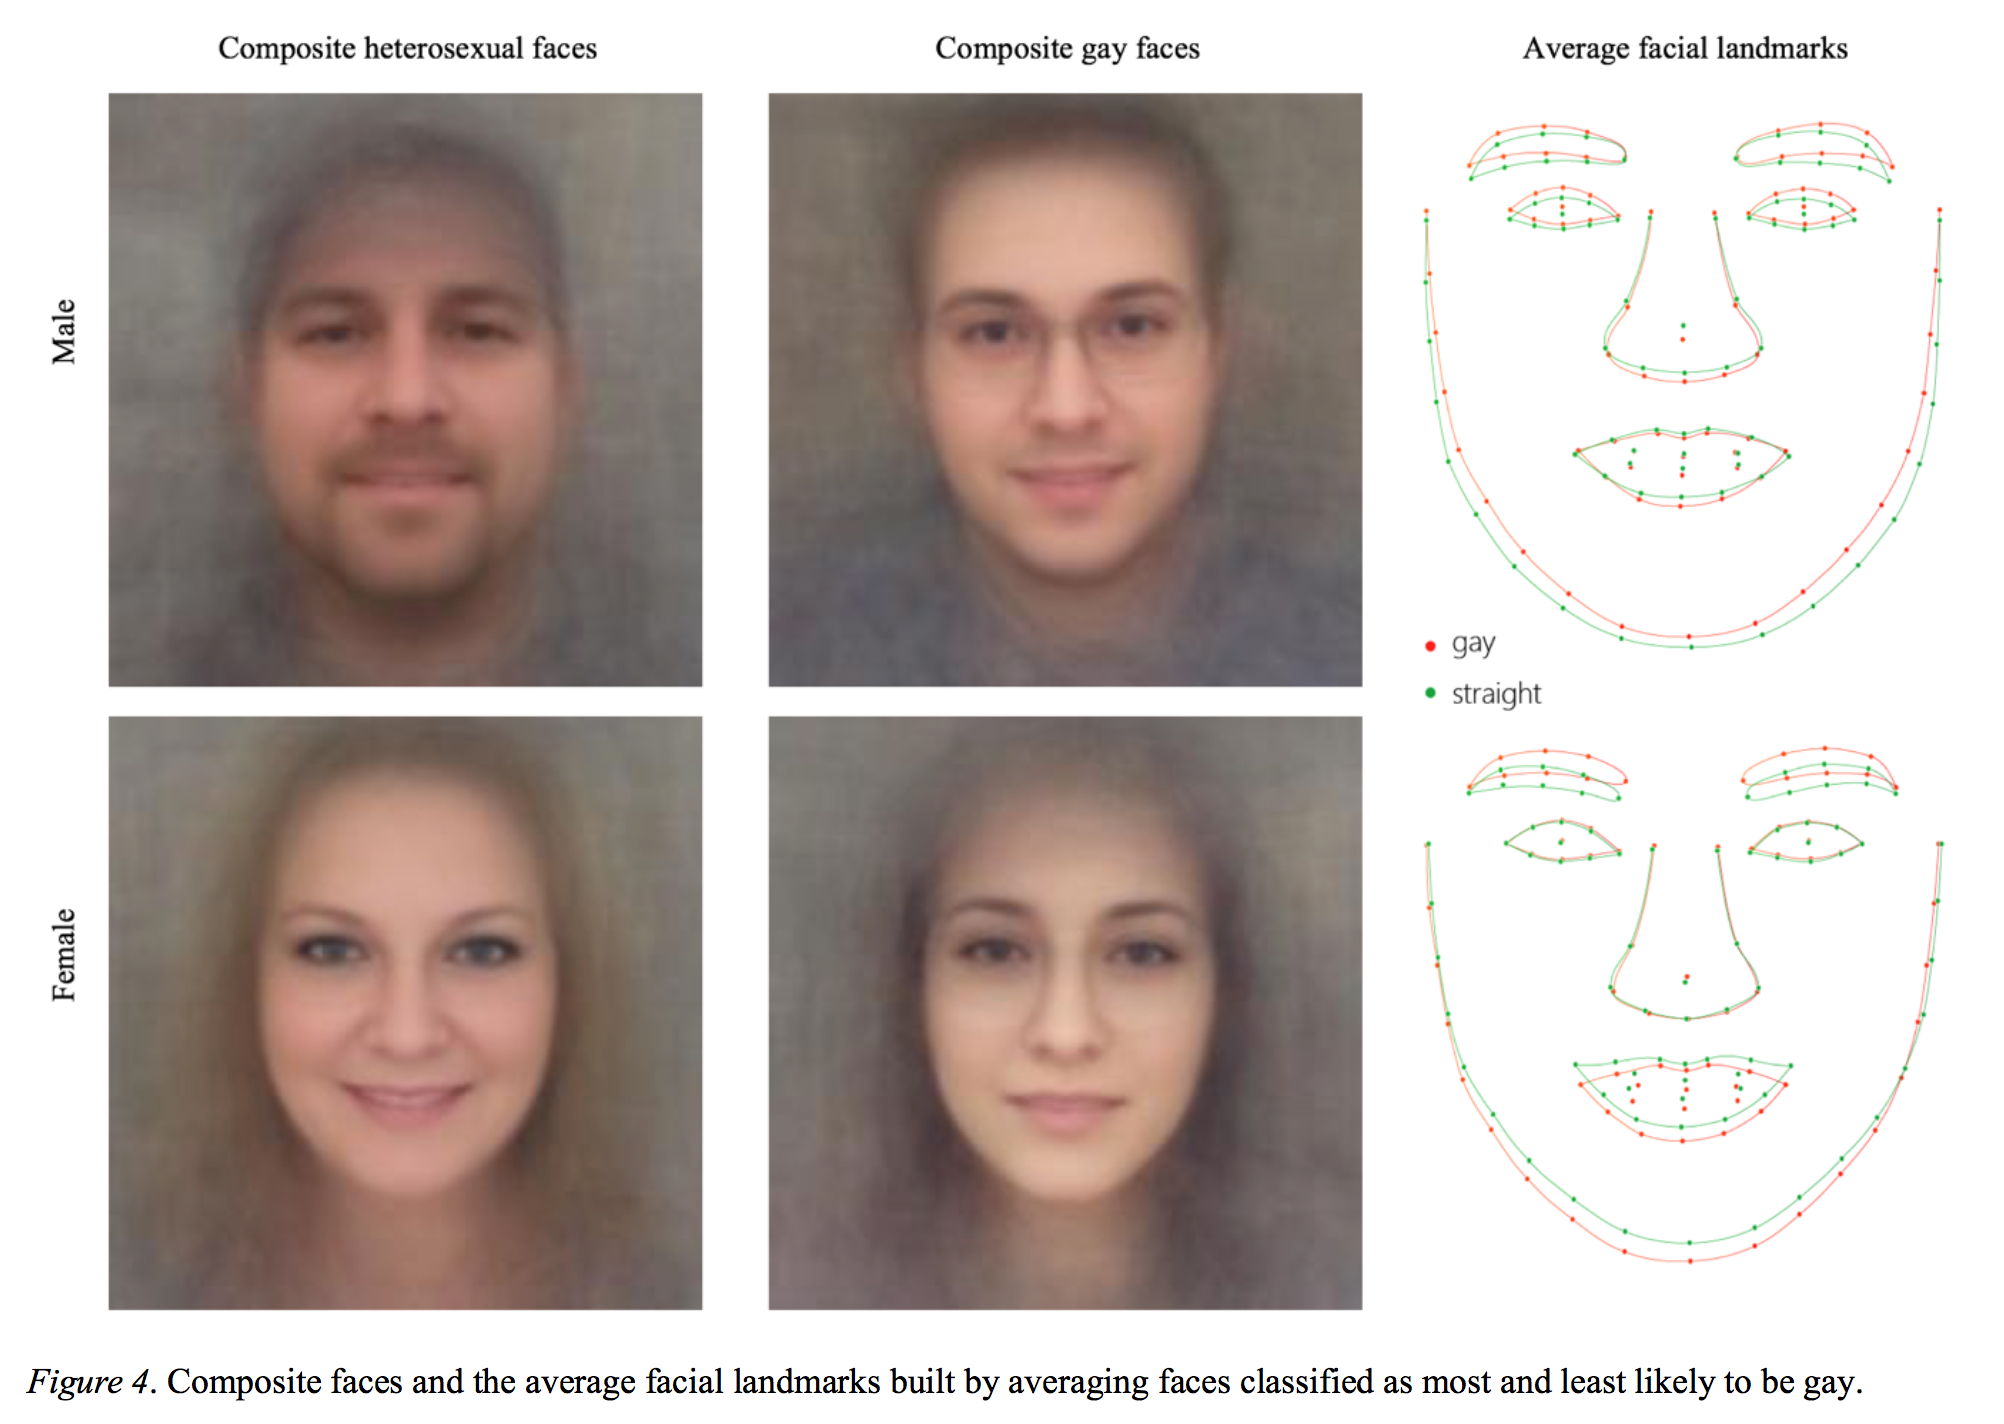
\includegraphics[width=\textwidth]{orientation3}
	\end{center}
\end{frame}

\begin{frame}
	\begin{center}
		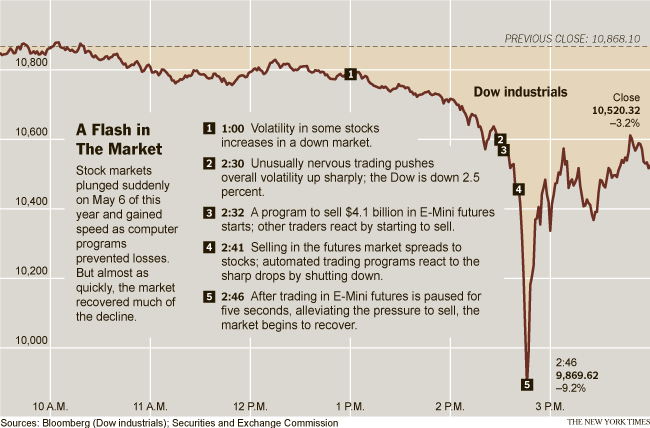
\includegraphics[width=\textwidth]{flashcrash}
	\end{center}
\end{frame}

\begin{frame}
	\begin{center}
		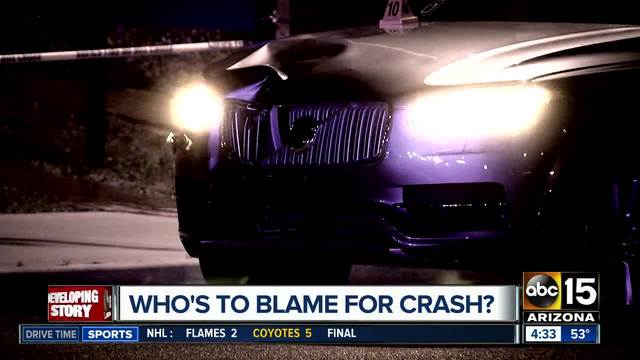
\includegraphics[width=\textwidth]{uber_tempe_2}
	\end{center}
\end{frame}

